\section{Liturgia chrzcielna}

\subsection{Procesja do baptysterium}
\begin{figure}[!hb]
	\centering
	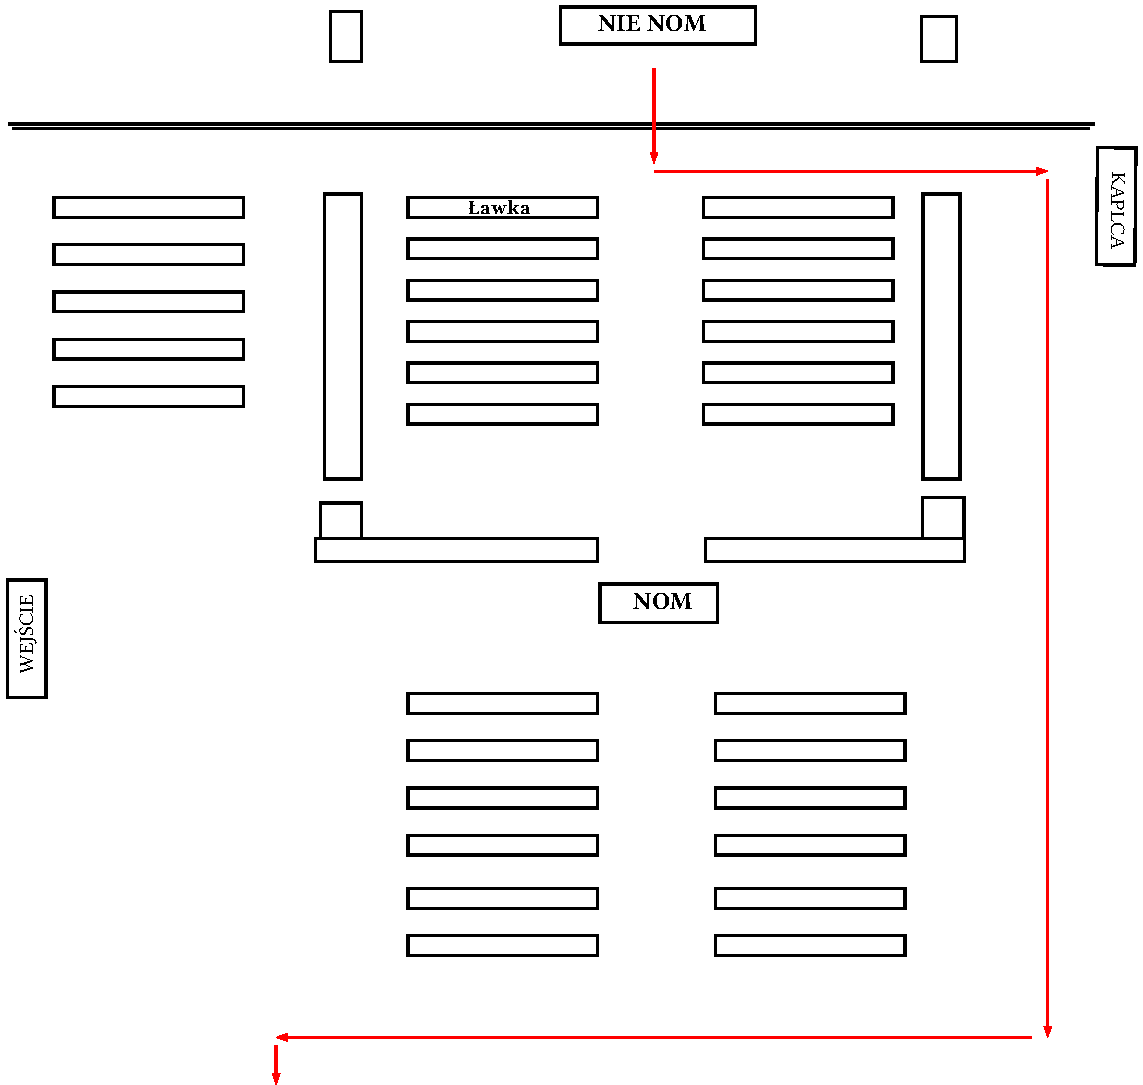
\includegraphics[width=0.55\linewidth]{procesja1.pdf}
	\caption{Droga do chrzcielnicy}
	\label{fig:procesja1}
\end{figure}
\begin{itemize}
	\item po ostatniej oracji \ii~ z \cc1 schodzi krótką drogą do sedilli,
	      ściąga \textcolor{violet}{fioletowy ornat i manipularz} (pomaga \zz~
	      \footnote{Orant zostaje wyniesiony do zakrystii -- na Mszy będzie
		      używany ornat \textcolor{red}{czerwony}}) i wkłada
	      \textcolor{violet}{fioletową kapę} (pomaga \cc2)
	\item w międzyczasie:
	      \begin{itemize}
		      \item kantorzy podejmują śpiew \textit{Sicut Cervus}
		      \item \aa\aa~ odpalają akolitki od znicza
		      \item \ding{63} idzie po krzyż procesyjny
		      \item \paschal~ idzie do Paschału \footnote{Paschał stoi na
			            stojaku poza prezbiterium} i go odpala \footnote{Można
			            to zrobić cieńką, woskową świeczką od znicza}
	      \end{itemize}
	\item na znak \cc1 formuje się procesja do chrzcielnicy:
	      \begin{center}
		      \cc2~~~\ii~~~\cc1 \smallskip\\
		      ministranci \smallskip\\
		      kantorzy \smallskip\\
		      \aa1~~~\ding{63}~~~\aa2 \smallskip\\
		      \cc3~~\paschal~~~~~~~ \smallskip\\
		      $\downarrow$
	      \end{center}
	\item procesja rusza na znak \cc1 (patrz Rys. \ref{fig:procesja1})
\end{itemize}
\subsection{Poświęcenie wody}
\begin{itemize}
	\item po dojściu do kraty:
	      \begin{itemize}
		      \item ministranci funkcyjni wchodzą do baptysterium (patrz Rys.
		            \ref{fig:woda})
		      \item chór też wchodzi do baptysterium, ale głębiej (koło drzwi
		            wejściowych) \footnote{Zostawiając przy tym miejsce dla
			            chóru, który musi stać bliżej chcielnicy} (patrz Rys.
		            \ref{fig:woda})
		      \item \ii, \cc1 i \cc2 stoją przed kratą (jeszcze nie patrz Rys.
		            \ref{fig:woda})
	      \end{itemize}
	\item \ii~ ściąga biret, podaje \cc1, ten odnosi i przynosi księgę z
	      modlitwą. \ii~ czyta kantyk \textit{Sicut Cervus} i czeka, aż chór
	      skończy jego śpiewanie. Następnie odczytuje oracje \smallfont{(złożone
		      ręce)} i po jej skończeniu wchodzi do baptysterium (teraz patrz Rys.
	      \ref{fig:woda})
	      \begin{figure}[h!]
		      \centering
		      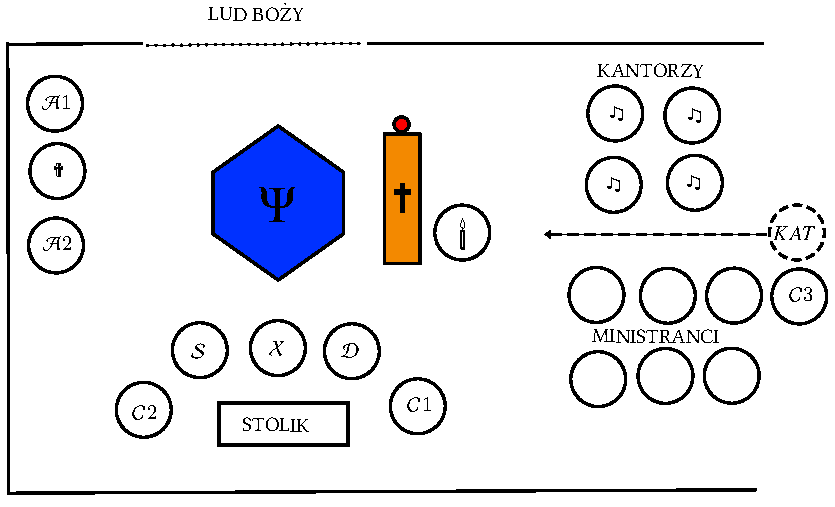
\includegraphics[width=0.7\linewidth]{woda.pdf}
		      \caption{Ustawienie przy chrzcielnicy, \spiew~ oznacza kantorów,
			      $KAT$ oznacza katechumena}
		      \label{fig:woda}
	      \end{figure}
	\item następuje poświęcenie wody chrzcielnej, \cc1 i \cc2 podtrzymują brzegi
	      kapy i pomagają \ii~ podając odpowiednie rzeczy (oleje, ręcznik \dots)
	      (patrz \textit{\nameref{sec:woda}})
\end{itemize}
\subsection{Chrzest}
\begin{itemize}
	\item \ii~ zmienia {\color{violet} fioletową kapę i stułę} na
	      \textcolor{black!50}{białą kapę i stułę}
	\item \cc3 wprowadza do baptysterium katechumenów z chrzestnymi (stoją oni
	      za ministrantami i kantorami)
	\item \ii~ rozpoczyna dialog z katechumenami
	\item po odpowiedziach na wszystkie pytania, \ii~ nad chrzcielnicą
	      trzykrotnie polewa głowę dziecka lub dorosłego, wypowiadając formułę
	      chrzcielną
	\item \cc1 podaje \ii~ naczynie z Krzyżmem. \ii~ namaszcza ochrzczonych
	      wypowiadając formułę i wyciera kciuk w watę
	\item następnie wręcza się białą szatę oraz płonącą świecę, wypowiadając
	      przepisane formuły
	\item następnie \ii~ wypowiada formułę: \textit{N., vade in pace...}
\end{itemize}
\subsection{Bierzmowanie}
\begin{itemize}
	\item kantorzy podejmują śpiew \textit{O stworzycielu Duchu Przyjdź}
	      % \item wszyscy oprócz \ii, \cc1, \cc2, \cc3 i \cc4 oraz \paschal~
	\item \ii~ w \textcolor{black!50}{białej kapie} z \cc1, \cc2, \cc3 (bierze ze sobą kropidło),
	      \aa1, \aa2, \ding{63} i \paschal~ (z Paschałem) udają się do kaplicy
	      św. Iwa, oddają rewerencje ołtarzowi i zajmują swoje miejsca:
	      \begin{itemize}
		      \item \ii~ siada na faldistorium
		      \item \cc1\cc2 stoją po bokach \ii~
		      \item \cc3 odkłada kropidło na kredencje i staje niedaleko
		            katechumena
		      \item \aa1 i \aa2 stoją przy kredencji, na której stawiają
		            akolitki
		      \item \ding{63} nie wchodzi do kaplicy ale stoi przed nią, po boku
		      \item \paschal~ stawia Paschał na stojaku i przy nim stoi
	      \end{itemize}
	\item przyprowadza się kandydata do ołtarza (razem ze świadkiem), którzy
	      klękają przed stopniem ołtarza po stronie epistoły
	\item po zakończeniu śpiewu następuje obrzęd bierzmowania (patrz
	      \textit{\nameref{sec:bierz}})
\end{itemize}
\subsection{Procesja do ołtarza głównego}
\begin{itemize}
	\item po skończonych obrzędach kantorzy \underline{niezłwocznie} podejmują
	      śpiew \textit{Litanii do Wszystkich Świętych} \footnote{Wszystkie
		      wezwania są śpiewane podwójnie}
	\item \ii~ zmienia \textcolor{black!50}{białą kapę i stułę} na
	      \textcolor{violet}{fioletową kapę i stułę}
	\item w międzyczasie formuje się procesja z powrotem do ołtarza głównego, w
	      tym samym porządku co poprzednio (ministranci nie funkcyjni wychodzą
	      zaraz po \aa\aa~ i \ding{63})
	\item po przybyciu do ołtarza:
	      \begin{itemize}
		      \item \paschal~ i \cc3 odstawiają Paschał na swoje miejsce (czyli
		            na stojak niedaleko stojaka na krzyż procesyjny) przy okazji
		            go gasząc
		      \item \aa\aa~ idą do kredencji
		      \item \ding{63} odkłada krzyż na stojak
		      \item reszta ministrantów idzie do chóru
		      \item \zz~ odbiera od \ii~ \textcolor{violet}{fioletową kapę} przy
		            stopniach ołtarza i odnosi ją do zakrystii
		      \item \cc1 i \cc2 stoją po bokach \ii
	      \end{itemize}
	\item \ii~ w \textcolor{violet}{fioletowej stule} kładzie się krzyżem na
	      stopniach ołtarza \todo{trzeba kiedyś położyć poduszki na
		      stopniach}, a wraz z nim klękają wszyscy ministranci (\cc1 i \cc2
	      po bokach \ii)
	\item na wezwanie \textit{Peccatores\dots} wszyscy wstają, formuje się
	      procesja \footnote{Nikt nie trzyma nic w rękach, a ksiądz idzie w
		      samej albie i stule} i wychodzi krótką drogą do zakrystii
	\item \ii~ ubiera \textcolor{red}{czerwony ornat i manipularz}, a
	      ministranci ubierają koronkowe komże
\end{itemize}
\subsection{Przygotowanie Mszy}
\begin{itemize}
	\item jak ministranci są jeszcze przy chrzcielnicy
	      \begin{itemize}
		      \item odstawić pulpit do kaplicy
		      \item ustawić relikwie, kwiaty
		      \item \textit{zmienić sedille} \todo{opcjonalnie}
	      \end{itemize}
	\item jak ministranci są już w kaplicy
	      \begin{itemize}
		      \item \textbf{zapalić 12 świec} (to zrobić jako pierwsze bo
		            najdłużej zajmuje)
		      \item zdjąć {\color{violet} fioletową} zasłonę z antypendium
		            \footnote{Tylko jeśli ludzie mogą oglądać tą zmianę}
		      \item odsłonić koronki
	      \end{itemize}
\end{itemize}

